\section{Aufbau der Spielarchitektur}
\label{sec:architektur}

\subsection{Überblick}
\label{sub:architektur:ueberblick}

Slick2D stellt Techniken zur Umsetzung eines zustandsbasierten Spieles zur Verfügung.
In Abbildung \ref{fig:spielarchitektur:states} werden die Zustände des Spiels und ihre Reihenfolge gezeigt.

Ein Spiel startet im \texttt{MainMenuState}.
Hier kann der Spieler das Spiel entweder direkt beenden oder in den \texttt{LevelMenuState} wechseln.
Der \texttt{LevelMenuState} bietet eine Auswahl aller zur Verfügung stehenden Levels an, welche dann im \texttt{PlayingState} gespielt werden können.
Während des Spiels kann das Spiel durch Wechsel in den \texttt{PauseMenuState} pausiert werden.
Nach erfolgreichem oder nicht erfolgreichem Abschluss eines Levels bietet der \texttt{GameFinishState} die Möglichkeit das Level zu wechseln, das Level erneut zu spielen oder das Spiel zu beenden.

\begin{figure}[]
\centering
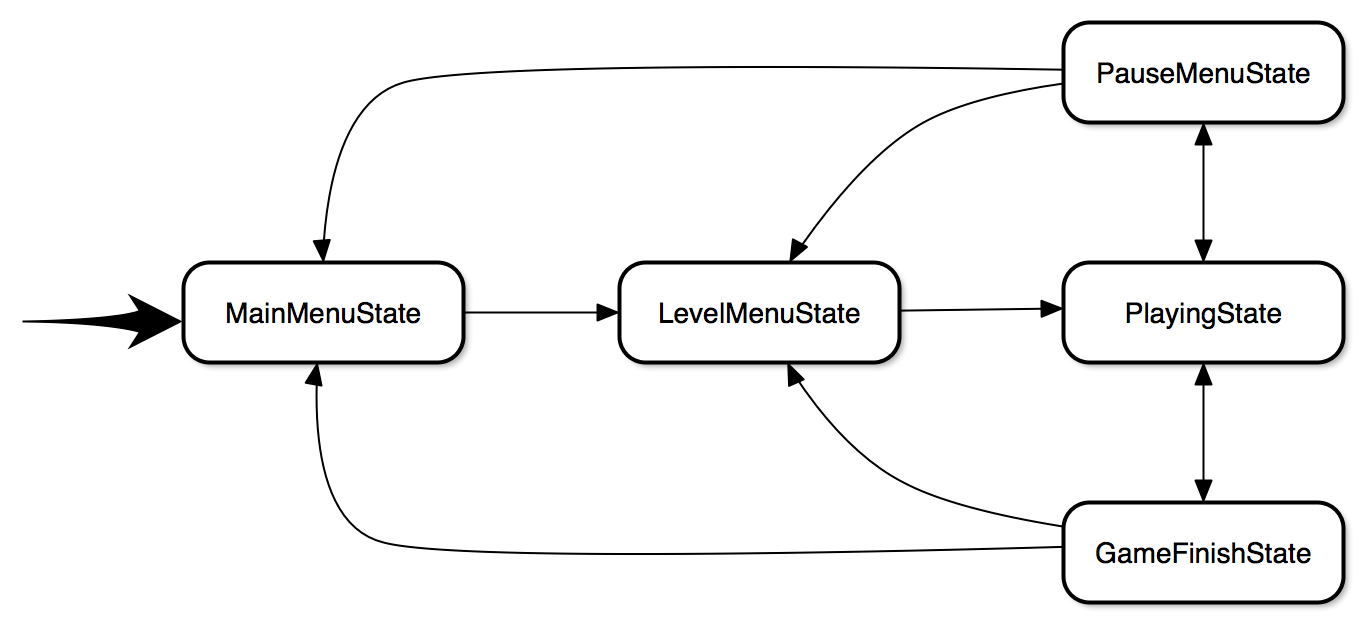
\includegraphics[width=3in]{img/05_states.png}
\caption{Übersicht der Zustände des Spiels}
\label{fig:spielarchitektur:states}
\end{figure}

Im FMC-Diagramm in Abbildung \ref{fig:spielarchitektur:fmc} wird die Bedeutung des \texttt{PlayingState} sowie der Aufbau eines Levels deutlich.
Der \texttt{PlayingState} empfängt die Eingaben des Spielers und reicht diese an den \texttt{LevelController} weiter.
Der \texttt{LevelController} kontrolliert und steuert die Bestandteile eines Levels.

\begin{figure}[]
\centering
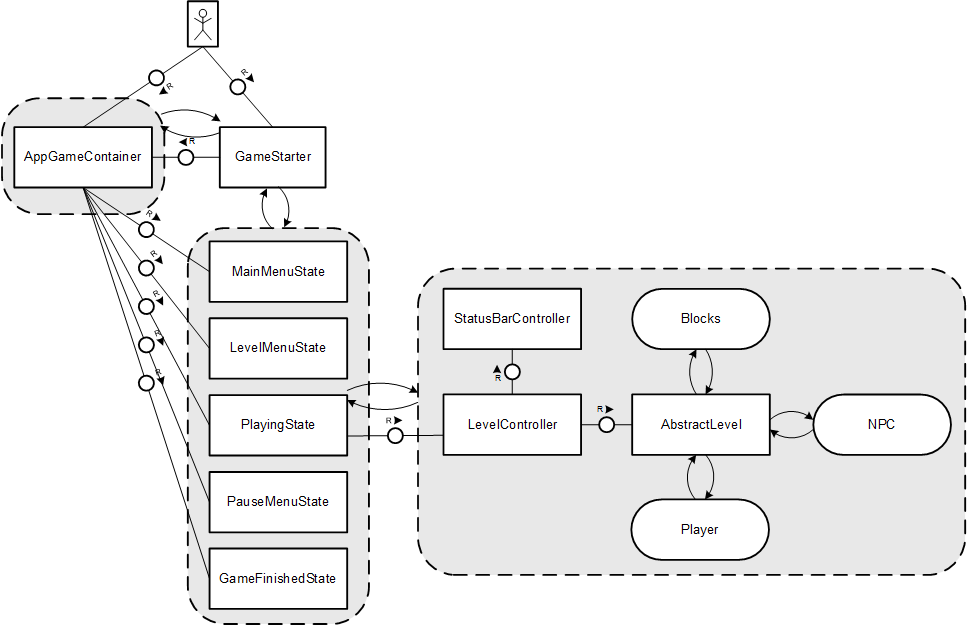
\includegraphics[width=3in]{img/05_fmc.png}
\caption{FMC Diagramm des Spiels}
\label{fig:spielarchitektur:fmc}
\end{figure}

\subsection{Level}
\label{sub:architektur:level}

Jedes Level erbt von \texttt{AbstractLevel}.
In Abbildung \ref{fig:spielarchitektur:abstractlevel} wird der Aufbau eines Levels deutlich.
Ein Level besteht aus einer Menge an \texttt{NPC}-Objekten (non-player character), welche die Gegner repräsentieren.
Außerdem beinhaltet es ein \texttt{Player}-Objekt sowie die Menge der Blöcke(\texttt{Block}), also der Karte des Levels.
Eine Übersicht über alle verwendbaren Spielobjekte wird in Abbildung \ref{fig:spielarchitektur:model} gegeben.
Level sind komplexe Datentypen und verstehen sich als Komposition der, in Abbildung \ref{fig:spielarchitektur:model} gezeigten, spielspezifischen \texttt{GameObject} Datentypen.
Zur Vermeidung von Redundanz und zur klaren Trennung zwischen Modell und Controller wird die Steuerung der Elemente eines Levels durch den \texttt{LevelController} übernommen.
Durch diese Trennung eignen sich Implementierungen von \texttt{AbstractLevel} sehr gut zur Erzeugung durch eine anwendungsspezifische Sprache.

\begin{figure}[]
\centering
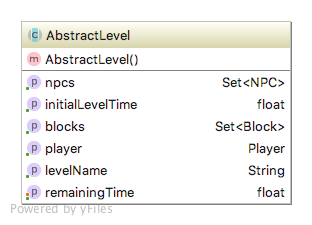
\includegraphics[width=2in]{img/05_abstractlevel_uml.png}
\caption{UML Darstellung der Klasse AbstractLevel}
\label{fig:spielarchitektur:abstractlevel}
\end{figure}

\begin{figure}[]
\centering
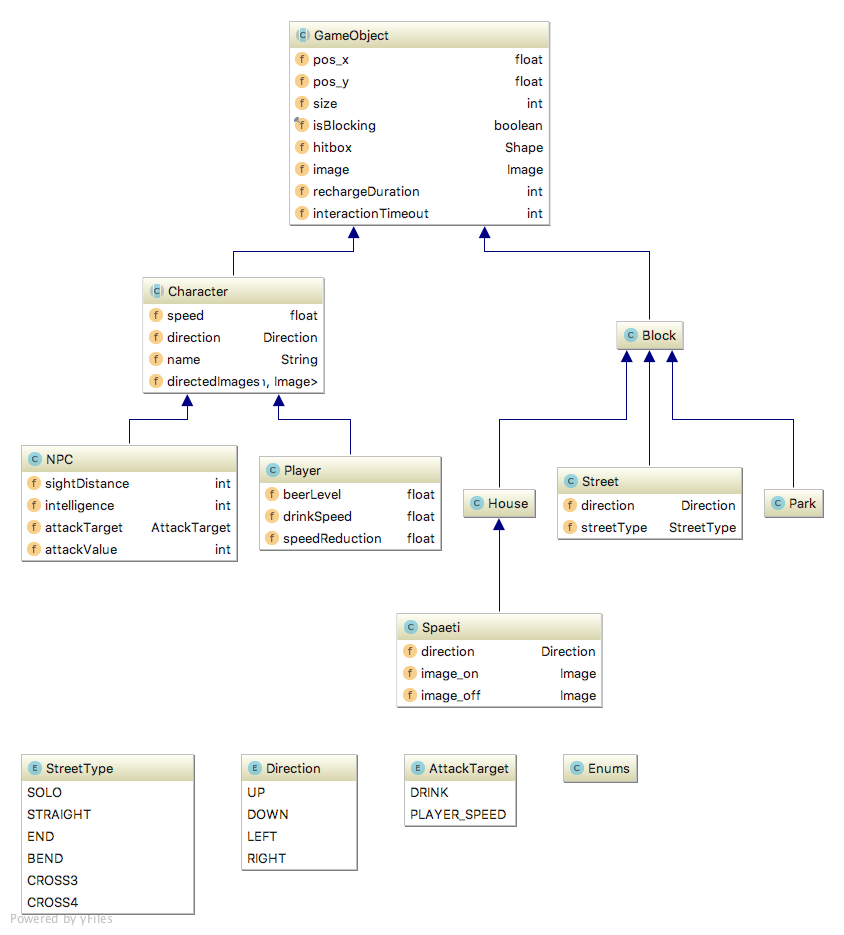
\includegraphics[width=3in]{img/05_model.png}
\caption{Spielobjekte}
\label{fig:spielarchitektur:model}
\end{figure}

\subsection{LevelController}
\label{sub:architektur:levelcontroller}

Der \texttt{LevelController} ist die funktionale Kernkomponente des Spiels.
Zu den wichtigsten Funktionalitäten zählen die Initialisierung eines Levels, die Kollisionskontrolle innerhalb eines Levels sowie die Berechnung der künstlichen Intelligenz der NPCs.
Auf diese Funktionalitäten wird im Folgenden näher eingegangen.

\subsubsection{Initialisierung des Levels}
In der Klasse \texttt{GameObject} in Abbildung \ref{fig:spielarchitektur:model} ist ersichtlich, dass jedes Spielobjekt Informationen über seine eigene Position auf der Spielfläche (\texttt{pos\_x} und \texttt{pos\_y}) besitzt.
Um die Level unabhängig von der Pixelgröße des Ausgabefensters und der Blockgröße zu gestalten, entsprechen diese Positionsangaben zunächst einfachen Indexwerten.
Die Indexwerte entsprechen der Position des entsprechenden Spielobjekts vom oberen linken Spielfeldrand aus.
Es werden zunächst alle Blockindexwerte mit den korrekten pixelbasierten Positionen aktualisiert.
In der aktuellen Implementierung weisen Blöcke der Karte eine feste Größe von 32x32 Pixeln auf.

Ebenfalls muss der Typ von \texttt{Street}-Objekten, also ob es sich hierbei beispielsweise um eine Kreuzung oder eine geraden Straße handelt, ermittelt werden.
Dazu wird während der Initialisierung eine Karte der Straßenobjekte in Form eines zweidimensionalen \texttt{boolean[][]}-Arrays erzeugt.
Anhand dieser Karte können nun, für jedes \texttt{Street}-Objekt einzeln, die Nachbarn ermittelt und der korrekte Straßentyp und eine eventuelle Rotation festgestellt werden.

\subsubsection{Kollisionskontrolle}
Der \texttt{LevelController} ermittelt Kollisionen zwischen \texttt{GameObject}-Objekten.
Dazu wird die Methode \texttt{Shape.intersect(Shape)} aus der Slick2D Bibliothek verwendet, welche zwei geometrische Objekte auf eine Schnittmenge untersucht und \texttt{true} zurück liefert sobald eine Schnittmenge existiert.
In diesem Fall berühren sich beide \texttt{GameObject}-Objekte und es wird auf beiden die \texttt{GameObject.interact(GameObject)} Methode aufgerufen.
Dies stellt die Interaktion zwischen zwei \texttt{GameObject} Instanzen sicher.
Innerhalb der konkreten Implementierungen von \texttt{interact()} wird dann unter anderem durch Reflection entschieden, welche Aktionen durchgeführt werden sollen.
In Listing \ref{lst:npc-interact} wird dies anhand der Implementierung der \texttt{interact()} Methode der Klasse \texttt{NPC} deutlich.
Sobald ein Objekt getroffen wird, welches die Eigenschaft \texttt{isBlocking} aufweist, wird eine Zufallsrichtung gewählt.
Wurde der \texttt{Player} getroffen, dann wird er, je nach spezifiziertem Angriffsziel, angegriffen und ein Timeout gesetzt um zu verhindern, dass Angriffe direkt nacheinander erfolgen können.

\begin{lstlisting}[caption={NPC.interact() Implementierung (NPC.java)}\label{lst:npc-interact},captionpos=t,language=Java]
@Override
public void interact(GameObject go) {
 if (go.isBlocking()) {
  this.setDirection(getRandomDirection());
 }
 if (interactionTimeout == 0) {
  if (go.getClass().equals(Player.class)) {
   Player p = (Player) go;
   if (attackTarget == Enums.AttackTarget.DRINK) {
    p.setBeerLevel(p.getBeerLevel() - attackValue);
    this.interactionTimeout = this.rechargeDuration;
   }
   if (attackTarget == Enums.AttackTarget.PLAYER_SPEED) {
    p.attackSpeed(attackValue);
   }
  }
 }
 super.interact(go);
}

\end{lstlisting}

Slick2D ist bestrebt, in regelmäßigen Abständen die implementierte Spiellogik durch Aufruf einer \texttt{update()} Methode zu aktualisieren.
Bei jeder Aktualisierung wird auf Kollisionen geprüft.
Es kann bei zu geringer Aktualisierungsrate, beispielsweise aus Performancegründen, oder zu hoher Geschwindigkeit der bewegenden Spielobjekte dazu kommen, dass einzelne Treffer mit Objekten nicht erkannt, und die Spielobjekte somit über Objekte springen können.
Aus diesem Grund unterteilt der \texttt{LevelController} Bewegungsintentionen in mehrere Teilschritte, prüft diese einzeln und unterbricht die Bewegung sobald eine Kollision innerhalb eines Teilschrittes erkannt wurde.
Dies sorgt auch dafür, dass Spielobjekte sauber an Kanten anderer Spielobjekte stehen bleiben und nicht beispielsweise wenige Pixel davor.


\subsubsection{Künstliche Intelligenz der NPC}
\label{subsub:architektur:ki}
NPC sind in der Lage ihr Umfeld wahrzunehmen und daraus Bewegungsänderungen abzuleiten.
Ihr Wahrnehmungsvermögen wird über zwei Kennzahlen gesteuert - Die Sichtweite und die ``Intelligenz''.
Die Intelligenz ist hierbei eine Wahrscheinlichkeit, mit der auf Wahrgenommenes reagiert wird.
Die \texttt{updateAI()} Methode iteriert über alle vorhandenen NPC und zieht jeweils eine Linie (Sichtlinie) zwischen dem entsprechenden NPC und dem Spieler.
Sofern die Sichtlinie kein optisches Hindernis (Blöcke mit \texttt{isBlocking} Eigenschaft) schneidet, wird geprüft ob die Länge der Sichtlinie im Bereich der Sichtweite des NPC ist.
Sofern dies der Fall ist, wird die beste Richtung zur Bewegung in Richtung des Spielers ermittelt.
Der NPC übernimmt diese Richtung mit der Wahrscheinlichkeit seiner Intelligenz.